\documentclass{beamer}
\usetheme{fibeamer}

\makeatletter
\renewcommand\fibeamer@includeLogo[1][]{}
\makeatother

\usepackage[utf8]{inputenc}
\usepackage[main=english, italian]{babel}

\def\mytitle{WiMAX LDPC codes}
\title{\mytitle} %% that will be typeset on the
\subtitle{Complexity and effectiveness} %% title page.
\author{Enrico Lovisotto}

\usepackage{ragged2e}  % `\justifying` text
\usepackage{booktabs}  % Tables
\usepackage{tabularx}
\usepackage{tikz}      % Diagrams
\usetikzlibrary{calc, shapes, backgrounds}
\usepackage{amsmath, amssymb}
\usepackage{mathtools}
\usepackage{url}       % `\url`s
\usepackage{listings}  % Code listings

\usepackage{color}

\frenchspacing
\begin{document}
\setbeamertemplate{caption}{\raggedright\insertcaption\par}
\frame{\maketitle}

\AtBeginSection[]{% Print an outline at the beginning of sections
  \begin{frame}<beamer>
    \frametitle{\mytitle}

    \tableofcontents[currentsection]
  \end{frame}}

\begin{darkframes}
  \section{Specification}
  \subsection{Design}
  \begin{frame}{Design}
  \end{frame}

  \subsection{Working modes}
  \begin{frame}{Working modes}
  \end{frame}

  \section{Simulation}
  \subsection{Encoder}
  \begin{frame}{Encoder}
    \begin{figure}[h]
      \centering
      
\includegraphics{figures/encoder.eps}
    \end{figure}
    \begin{equation*}
      c_i = ENC(u_i) =
      \left[
          \begin{array}[h]{c|c}
            u_i & A u_i
          \end{array}
        \right]
      \quad \text{where} \quad  \begin{dcases}
        H = \left[
          \begin{array}[h]{c|c}
            B & C
          \end{array}
        \right] \\
       A = C^{-1} B
      \end{dcases}
    \end{equation*}
  \end{frame}

  \subsection{Modulator and channel}
  \begin{frame}{Modulator and channel}
    \begin{figure}[h]
      \centering
      
\includegraphics{figures/channel.eps}
      \label{fig:channel_model}
    \end{figure}
    \begin{equation*}
      \begin{split}
        d_i
        = MOD(c_i)
        = & \begin{dcases}
          +1 & c_i = 1 \\
          -1 & c_i = 0
        \end{dcases} \\
        r_i
        = d_i + w_i \quad\text{where}\quad
        & \begin{dcases}
          w_i \sim \mathcal{N}(0, \sigma^2) \\
          \sigma^2 = \left( 2R~ \frac{E_b}{N_o} \right)^{-1}
        \end{dcases}
      \end{split}
    \end{equation*}
  \end{frame}

  \subsection{Decoder}

  \begin{frame}{Function $\tilde{\phi}$}
    \begin{figure}[h]
      \centering
      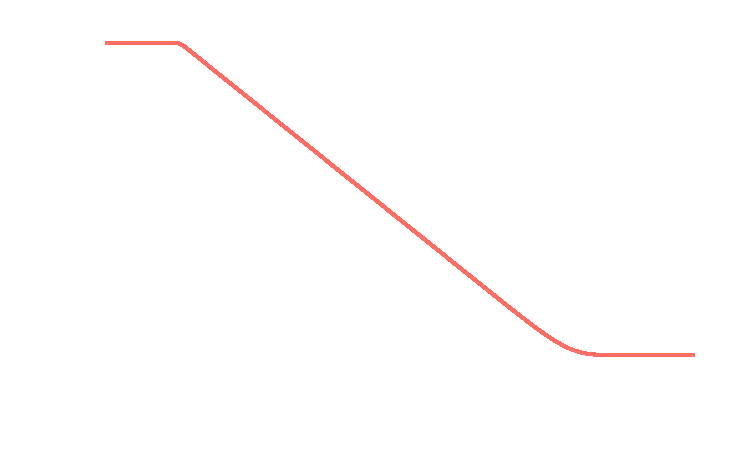
\includegraphics[width=\textwidth]{../plots/figures/phi_tilde.pdf}
      \vspace{-1cm}
      \caption{Function is approximated for small and high values of $x$}
      \label{fig:phi_tilde}
    \end{figure}
  \end{frame}

  \begin{frame}{Sparse matrices}
    % data structure + performances
    % specific operations implemented
    \begin{figure}[h]
      \centering
      
\includegraphics[width=\textwidth]{figures/sparse-matrix.eps}
      \caption{In-memory representation of a generic matrix $A$}
      \label{fig:phi_tilde}
    \end{figure}
  \end{frame}

  \definecolor{my-orange}{HTML}{FFCD64}
  \definecolor{my-green}{HTML}{92FF64}
  \definecolor{my-purple}{HTML}{B164FF}
  \definecolor{my-blue}{HTML}{64C3FF}

  \begin{frame}{Message passing}
    \begin{minipage}{0.7\linewidth}
      \begin{figure}
        \hspace{-1cm}%
        
\includegraphics[scale=1.4]{figures/message-passing.eps}
        \caption{FFG of a generic LDPC code}
        \label{fig:phi_tilde}
      \end{figure}
    \end{minipage}%
    \begin{minipage}{0.4\linewidth}
      ~~ $\textcolor{my-orange}{ch}$ channel information

      ~~ $\textcolor{my-blue}{F}$ forward messages

      ~~ $\textcolor{my-purple}{B}$ backward messages

      ~~ $\textcolor{my-green}{b}$ extrinsic information
    \end{minipage}
  \end{frame}

  \section{Results}
  \subsection{Code length}
  \begin{frame}{Code length}
  \end{frame}

  \subsection{Code rate}
  \begin{frame}{Code rate}
  \end{frame}

  \subsection{Message passing iterations}
  \begin{frame}{Message passing iterations}
  \end{frame}

  \subsection{Message passing algorithm}
  \begin{frame}{Sum-product VS other}
  \end{frame}

\end{darkframes}

\end{document}

%%% Local Variables:
%%% mode: latex
%%% TeX-master: t
%%% End:
